%% Settings for single-side (simplex) printing
% Margins: left 40mm, right 25mm, top and bottom 25mm
% (but beware, LaTeX adds 1in implicitly)
\documentclass[12pt,a4paper]{report}
\setlength\textwidth{145mm}
\setlength\textheight{247mm}
\setlength\oddsidemargin{7.5mm}
\setlength\evensidemargin{7.5mm}
\setlength\topmargin{0mm}
\setlength\headsep{0mm}
\setlength\headheight{0mm}
% \openright makes the following text appear on a right-hand page
\let\openright=\clearpage

%% Character encoding: usually latin2, cp1250 or utf8:
\usepackage[utf8]{inputenc}

%% Prefer Latin Modern fonts
\usepackage{lmodern}

\usepackage{amsmath}        % extensions for typesetting of math
\usepackage{amsfonts}       % math fonts
\usepackage{amsthm}         % theorems, definitions, etc.
\usepackage{bbding}         % various symbols (squares, asterisks, scissors, ...)
\usepackage{bm}             % boldface symbols (\bm)
\usepackage{graphicx}       % embedding of pictures
\usepackage{fancyvrb}       % improved verbatim environment
\usepackage{natbib}         % citation style AUTHOR (YEAR), or AUTHOR [NUMBER]
\usepackage[nottoc]{tocbibind} % makes sure that bibliography and the lists
			    % of figures/tables are included in the table
			    % of contents
\usepackage{dcolumn}        % improved alignment of table columns
\usepackage{booktabs}       % improved horizontal lines in tables
\usepackage{paralist}       % improved enumerate and itemize
\usepackage[usnames]{xcolor}  % typesetting in color
\usepackage{float}
\usepackage[boxruled]{algorithm2e}
\usepackage{gensymb}

\usepackage{enumitem}
\usepackage{courier}
\usepackage{epstopdf}
\begin{document}

% TITLE PAGE
\begin{titlepage}
    \begin{center}
        \vspace*{1cm}
        
        \Huge
        \textbf{Pepr3D}

        \LARGE
        
        \vspace{12cm}
        
		\Large
        \textbf{Authors}: Bc. Štěpán Hojdar,
                Bc. Tomáš Iser,       
        Bc. Jindřich Pikora,
		Bc. Luis Sanchez
		\\
		\textbf{Supervisor}: Mgr. Oskár Elek, PhD.
		\\
		\textbf{Consultants}: doc. Ing. Jaroslav Křivánek, Ph.D., Ing. Vojtěch Bubník (Prusa Research s.r.o.)
        
        \vfill

		Faculty of Mathematics and Physics \\	
		Charles University		               
    \end{center}
\end{titlepage}

%% TOC
\setcounter{tocdepth}{1}
\tableofcontents

% TODO: Stepan
\part{Introduction and Functional Requirements}
\chapter{Introduction}

\section{3D printing basics}

3D printing is a new technology that has seen rapid developement in the last years. It comes in many different forms, melting plastic, fusing metals, shining UV on photopolymers, etc. Fused Deposition Modelling (FDM) is the most popular and accessible to the general public and for the purpose of this project, when we talk about 3D printing, we will always mean FDM printers, unless stated otherwise.

FDM printing is a relatively simple process - a printer head melts the plastic filament and deposits it on a preheated platform layer by layer, from the bottom towards the top. The printer has to regulate the temperature of both the filament in the head and the moving platform for the deposited material to bond correctly. Several types of filaments are used, namely PLA, ABS, PET and others.

\section{Prusa environment}

The Prusa environment is very similar to the general description we provided in the section 1.1. For the puprose of our project, the most important concept in the Prusa environment is the slicer. The slicer is a program that receives the 3D model the user wishes to print out and creates the instructions for the Prusa 3D Printer -- a G-code file. The file is then transfered to the printer, which then executes the commands in the G-code file. The slicer has to plan the movement of the head for the whole print. This includes several crucial things:

\begin{itemize}
\item Covering the whole area of each layer
\item Reinforcing the walls of the object to make them sturdier
\item Filling the inside of the object with a rougher print, because it won't be visible when finished
\item Planning the path so the head can stay in one Z level - an "Eulerian path".
\item Switching the materials for multimaterial printing (more in 1.3)
\end{itemize}

Prusa develop their own slicer - a forked branch of an open-source program called Slic3r \footnote{http://slic3r.org/}, called Slic3r Prusa Edition \footnote{https://www.prusa3d.com/slic3r-prusa-edition/}. This slicer can do all we listed above very well.

\section{Multimaterial printing}

Multimaterial printing is a very new concept, even in the fairly new world of 3D printing. Many of the simpler and cheaper 3D printers can only print one material models - one color for the whole object. However, many users would like to print models that include more than one color. Even though the more advanced printers are capable of combining up to four different materials into one print, the process to achieve this is rather cumbersom for the end user - the user has to manually split the 3D mesh of the object into parts that he wishes to have a different color.

For example, if we are printing a dragon, want the dragon to be black and have white teeth, we have to take the dragon model, and split off each individual tooth. Then tell the slicer that the remaining file - the toothles dragon should be black and the teeth should be white.

This model splitting has to be done in a full 3D editing software like Blender or 3ds Max, which is difficult to control for newcomers and overly complex.

\section{Our project}

Our project aims to make printing a multi-colored object a lot easier, by developing an application that will allow the user to simply paint on the 3D model (i.e. the dragon) with different colors (i.e. color the teeth white), then simply click export and generate the files of the split-off models automatically.

Our application should allow for free hand painting as well as some forms of guided painting - bucket fill and some smarter tools, for example a bucket fill that studies the object's geometry and stops the filling if it detects a sharp edge (i.e. the transition of the tooth into the dragon).

Our aim is to make the application for desktop PCs, with main developement time being focused on the Windows operating system. However, we are trying to use software engineering tools that can also be ported to a plethora of other platforms like Linux based OS, Mac OS and mobile, if the need should arise.

\section{Related works}

Based on the analysis of the experts from Prusa Research s.r.o, there, at the moment, does not exist a software that does what this project is trying to achieve.

The closest existing software is Autodesk Meshmixer \footnote{http://www.meshmixer.com/}, which is very complicated and is not targeted for FDM printing specifically. As such, it includes a lot of features that are not important for the FDM users and end up being confusing.

Microsoft 3D Builder \footnote{https://www.microsoft.com/en-us/p/3d-builder/9wzdncrfj3t6?activetab=pivot\%3Aoverviewtab} is another application that handles 3D models but we have not found a way to make it create anything remotely applicable to FDM printing.

Any 3D computer graphics program designed to handle 3D models which allows for the model to be created or split by colors manually. This section would include software as 3ds Max, Maya or Cinema4D. Using these applications, however, would be very time comsuming for the user and practically unusable on a larger scale.

\section{Challenges in this project}

This section should briefly familiarize the reader with some of the parts of the application we think will be difficult to implement correctly, before we present the full program specification.

\subsection{Handling the geometry during editing}

We want our application to be able to emboss text on the surface of the object, detect edges and stop painting the color during bucket fills, allow the user to paint fine details on a rough triangle mesh. All of these things require some degree of subdividing the triangle mesh to allow the user to create small details. We think that this potentially could involve some difficult problems - we have to allow the user to subdivide the triangle mesh enough to actually allow him to create fine details on the surface. However, the if the user goes overboard with the subdivision, the model will be too complex to print or even handle inside a desktop PC.

\subsection{Exporting the finished objects}

After the user is done painting, the application will have to separate the designated objects and areas into distinct meshes. This is potentially a very complicated task to do correctly for non-convex meshes. For example: if we are writing a text on a ball, we really only want the text to be carved deep enough into the ball for the printed material to hold firmly, we do not want it to be too deep. However, if we want the dragon's teeth to be white, we would prefer the whole tooth to be white, not just its surface. The distinction between these two cases could be non-trivial.

\subsection{Performance}

Handling complex geometry is a very taxing task for the user's computer. This application is targeted on beginner-level customers of simple and non-expensive 3D printers. Therefore the application cannot be too hardware demanding -- it has to run smoothly on an average 3 year old PC or laptop. We expect it is going to be hard to ensure this is the case.




\chapter{Use case}

\section{Wireframe of the application}

Figure \ref{fig:wireframe} provides a simple wireframe sketch of the application graphical user interface (GUI). The window consists of several usual components:
\begin{itemize}
\item A horizontal toolbar at the top, allowing for a fast selection of tools and file manipulation
\item A 3D preview window, with live preview of the object. This window allows rotating and magnifying the object, as well as the application of selected tools (e.g. painting with a brush). A simple grid and a 3D cross is provided to ensure the user is always aware of object orientation, as it is important for 3D printing.
\item An options window on the right allows the user to customize the settings of the currently selected tool (e.g. selecting the color for a brush).
\end{itemize}

\hspace{-30pt}
\begin{figure}
	\centering
	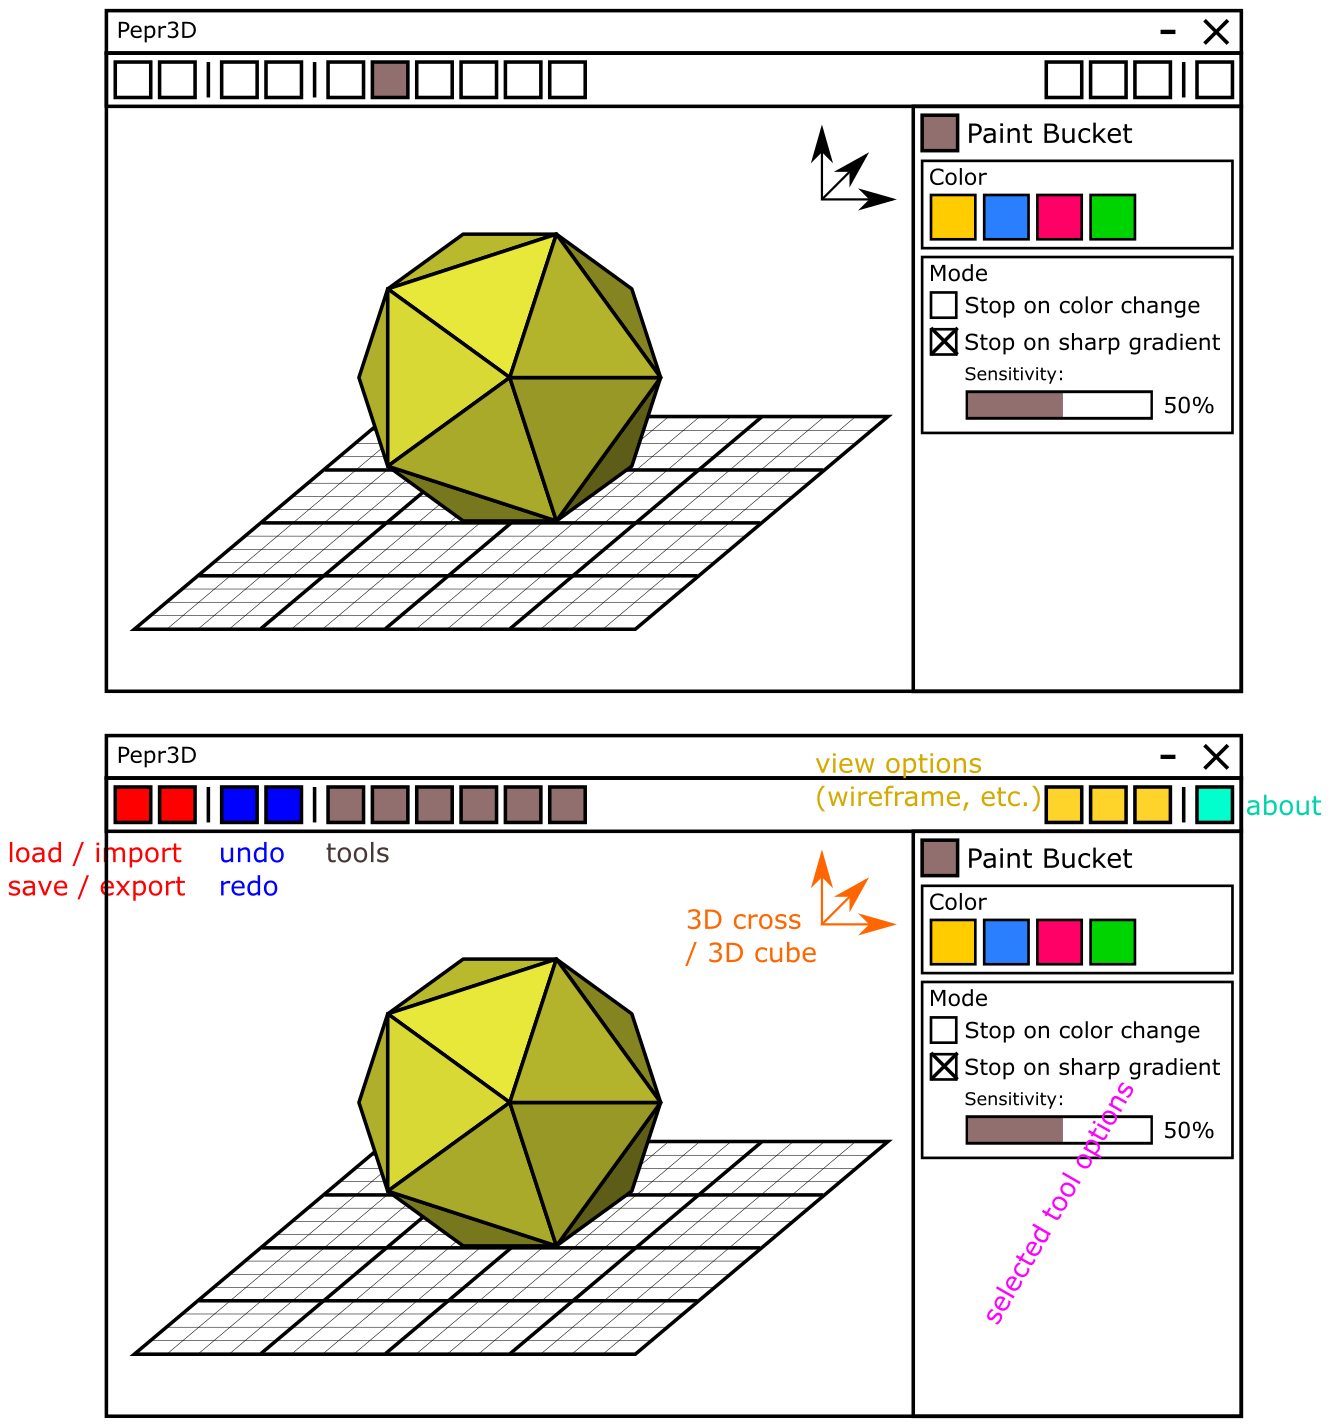
\includegraphics[scale=0.35]{images/wireframe.png}
	\caption{A simple wireframe sketch of the application.}
	\label{fig:wireframe}
\end{figure}

\section{Workflow}

In this section we describe the intended workflow for a user who has a 3D model he wishes to color and then print on a multicolor FDM printer. This application is intended for users of varying degrees of experience and our goal is to create as easy-to-use application as possible.

\subsection{Importing the model}

First, the user has to import the model he found or created. Clicking on the \textit{import button} creates a dialog, the user selects the 3D model and the model gets loaded. The application should accept at least a few standard formats -- namely Wavefront $.$obj and $.$stl \footnote{https://en.wikipedia.org/wiki/STL\_(file\_format)}, both of which are widespread and well known among the 3D printing community.

The user should also be able to continue on an already existnig project made earlier with Pepr3D.

After the model is loaded, it will be rendered in the 3D preview window. The window allows the user to rotate, zoom in and out and preview the wireframe of the model (rendering only edges and no faces of the model). The user is able to set the number of colors he wants to use (by default $4$ because current Prusa printers support up to four colors). The model is colored with the first color by default.

The user then selects one of the tools from the toolbar. This will bring up the \textit{Tool options} menu on the right hand side allowing the user to customize the tool.

\subsection{Tools}

\subsubsection{Edit history}
%TODO nafukovací feature
The user is always able to revert his last action by using an \textit{Undo button} or a keyboard shortcut. Depending on the technical difficulties, this feature could also persist through different sessions.

\subsubsection{Save as Pepr3D project}
Saves the current project as a Pepr3D project file. Upon re-opening Pepr3D, the user can load the project back and continue the work as if he never left. Does not include exporting the file into a slicer-compatible format.

\subsubsection{Export}
Export the file into a slicer-compatible format. This file is then handed to the slicing program (e.g. Slic3r Prusa Edition we mentioned earlier) and can be printed directly.

\subsubsection{Triangle painter}
After selecting a color, the user can assign said color to triangles he clicks on. Backside filtering is always on, so the user can only ever color a triangle that faces towards him, which should prevent a lot of accidents a lesser experienced user might make.

\subsubsection{Bucket painting}
The user selects a color and by clicking anywhere on the model paints all triangles with selected color until an edge criterion is met. The simplest and most intuitive edge criterion is continuity (a hole stops the bucket spread). Several more criterions could be useful when in 3D, namely the sharpness of the normal (if two neighbouring triangles are at an angle greater than $X$, stop.) or a big gradient in a \textit{shape diameter function} (SDF).

\subsubsection{Automatic segmentation}
Pepr3D fully automatically colors the whole model using the selected colors, according to a edge criterion as discussed in the \textit{Bucket painting} section. The user can then decide if he wants to merge some segments together, reducing the number of colors.

\subsubsection{Semi-automatic segmentation}
The user roughly paints over triangles in areas that should have distinct colors, as indicated by Figure \ref{fig:rabbit}. The program then finishes the coloring by executing a clever flood-fill algorithm utilizing SDF, sharp edges, etc. 

\begin{figure}
	\centering
	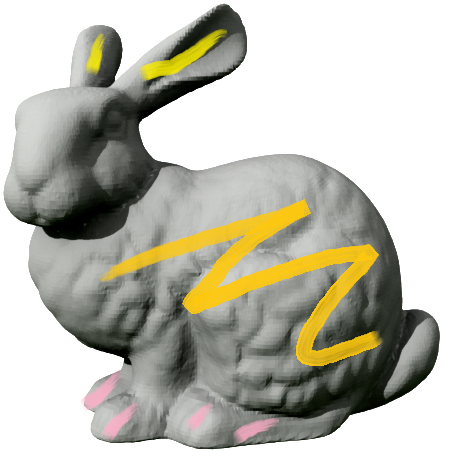
\includegraphics[scale=0.75]{images/rabbit.png}
	\caption{Semi-automatic segmentation as seen from the user's perspective. The ears of the rabbit are yellow as indicated by one stroke on each ear. The body is orange as indicated by the stroke on its back. The rabbit's feet are pink -- four pink strokes.}
	\label{fig:rabbit}
\end{figure}

\subsubsection{Brush}
A simple to use brush tool that allows to paint onto the model with a selected color. This tool allows the user to paint finer details, even though the geometry does not include them. For example painting the nose of the rabbit from Figure \ref{fig:rabbit} black -- there is no distinct edges on the nose, but the user can color only the nose by fine strokes of the brush.

The implementation of this tools is harder, because the program needs to adaptively subsample the triangle mesh to allow for finer details. This poses a lot of problems, which will later be discussed in the implementation parts of the document.

\subsubsection{Text}
Using the \textit{tool options} window, the user selects a font and types a custom text into a window. The text gets projected onto the model using some sort of projection transformation (customizable by the user from a limited range of projections). The software also allows extruding the projected text in the direction of the surface normal to create a $3$D effect.

\subsubsection{Triangle subdivision/decimation}
The user selects a section of triangles and then presses either subdivide or decimate, which will either make the geometry more complicated (and smooth), or simpler and more rough. See Figure \ref{fig:decimated} for visual aid.

\begin{figure}
	\centering
	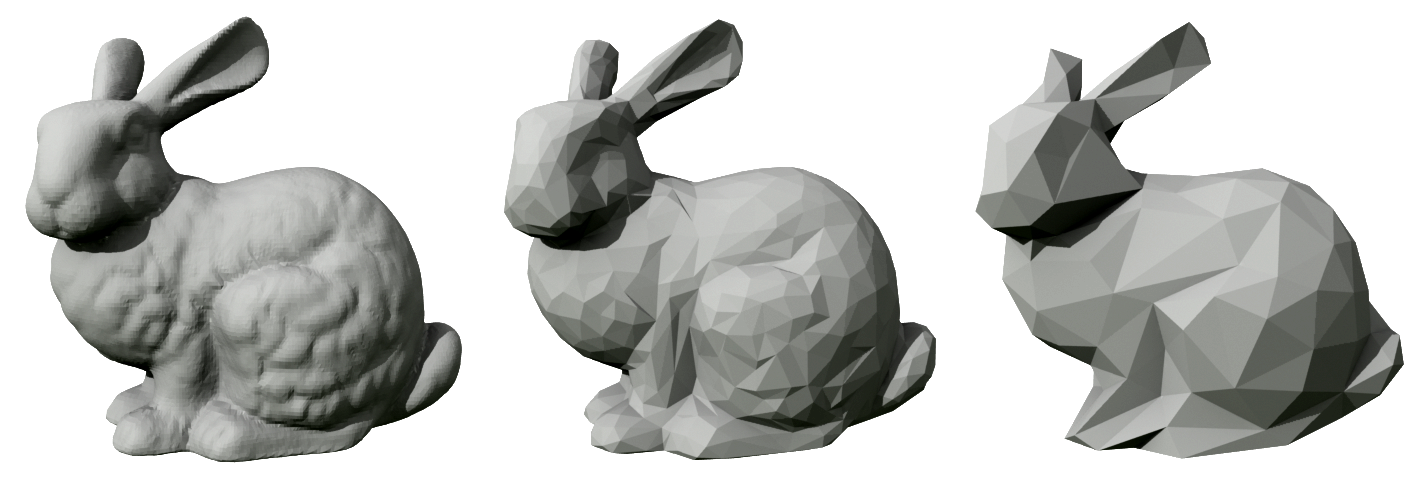
\includegraphics[scale=0.25]{images/decimated_bunny.png}
	\caption{Three stages of triangle numbers. The bunny on the left has the most triangles and most complicated geometry. Several decimations can reduce the number of triangles but also the number of details as shown on the second and third bunny.}
	\label{fig:decimated}
\end{figure}



\part{Non-Functional Requirements}
\chapter{Architecture}

TODO by Tomáš
\chapter{Core modules}

\begin{figure}[b]
	\centering
	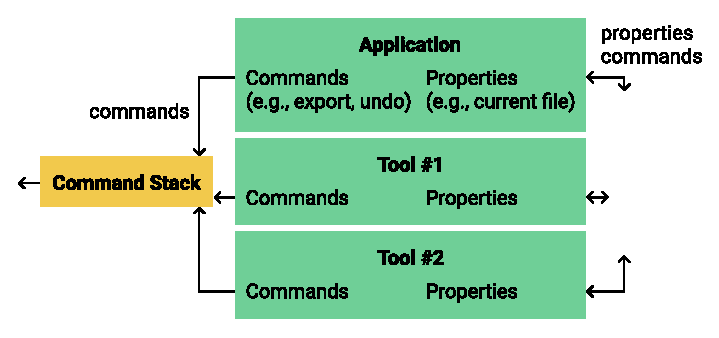
\includegraphics[scale=0.9]{images/architecture_commandstack}
	\caption{The part of architecture covered in this chapter.}
	\label{fig:architecture_commandstack}
\end{figure}

This chapter takes a closer look at the portion of the architecture higlighted in Figure \ref{fig:architecture_commandstack}. We will explain how each task is performed once the UI element has received the input from the user. The UI portion of the architecture will be covered in the next chapter.

% TODO: WARNING: CAREFUL, JE UI NEXT NEBO PREVIOUS CHAPTER?

\section{Commands}
Commands are the primary means of altering the geometry model. Each of them gets executed and placed on the command stack, which allows for the \textit{Undo and Redo} operations to function correctly. The commands then interact with the geometry model (this interaction will be explained in greater detail in the chapter regarding the geometry model) to modify it according to the user's wishes.

Because each command gets put on the command stack, and each Undo step removes one command from the stack, each command has to have a visual impact on the user's work. This means that internal computations, such as geometry queries, cannot be represented as commands, because pressing the Undo button would not have any visual effect and would confuse the user. Examples of commands include: coloring a single triangle (triangle painter tool), adding a brush stroke (as in semi-automatic segmentation we looked at in Chapter 2) or a single step of triangle mesh subdivision.

\subsection*{Implementation details}

A command will be a class with three primary methods.
\begin{itemize}
\item \textit{constructor} -- Once the command gets created, the main thing to do is remember the state the geometry model was in before the command modified it. This will allow for the command to restore the model if \textit{Undo} is pressed. The advantage of saving the state in the constructor and not in the execute function itself is because of the \textit{Redo} mechanism -- if the user repeatedly presses the combination of \textit{Undo + Redo}, the model gets saved only once as opposed to each execute.
\item \textit{execute()} -- The execute function will perform the task the command is created to do. This will typically get called immediately before the command gets placed onto the command stack.
\item \textit{undo()} -- This method will take the state of the model saved by the constructor of the command and apply it to the current geometry model, effectively reversing the command.
\end{itemize}

\section{Command Manager and Command Stack}

\subsection{Command Stack}

As the name suggests, the Command Stack is a \textit{LIFO} type structure, its main purpose to store the executed commands to allow for the \textit{Undo and Redo} operations to be performed. As we have outlined in the previous section, each command carries all neccessary information to perform both actions. This means that the Command Stack can be a simple container without any significant logic behind it.

\subsection{Command Manager}

The command manager is a object to manage the command stack. It receives the commands from tools, executes them and stores them in the command stack. When the user wishes to \textit{Undo} an operation, the command manager retrieves the top command from the stack and invokes its undo() method.

\section{Tools}

A tool is the main programable component which connects the low-level command structure we outlined above and the high-level UI components (such as color-pickers, the user performing brush strokes and file operations like exporting the file). This design should also allow for later advancements of the software easily -- adding a tool to the software should be a matter of writing the new tool's Tool class, unless the tool is advanced and needs some complicated custom geometry processing functions.

Each tool is composed of two main components:
\begin{itemize}
\item \textit{properties} -- a methodless object holding the tool's properties which can be customized by the user. This includes, for example, the color which gets assigned to the triangles in the triangle painter tool, the number of colors for automatic-segmentation, the subdivision level or the gradient thresholds for region detection in bucket painting. The information in this object gets changed directly when the user interacts with the UI.

\item \textit{commands} -- Each tool generates at least one command, which it creates, fills with all neccessary information the command needs to execute itself, and passes it to the command manager. More complicated tools can create more commands, as we will illustrate in the following section. The tool is able to do some pre-processing before a command is issued, in case the pre-processing isn't visible on the screen, as shown in example 4.1.

\end{itemize}

\section{Examples of data flow within the center section of the achitecture}

We include a few example use cases which should illustrate what happens in the application (normal font) when a user interacts with the UI (italics). The first example shows the need for preprocessing power within the tool class, while the second example illustrates the need for multi-command tools.

\subsection{A preprocessing example - triangle painter}
\textit{The user selects the triangle painter from the tool box, and in the Side Pane, he changes the color from default red to green.}

This action makes the UI manager change the color property of the TrianglePainter tool from red to green.

\textit{The user then clicks on a triangle that he sees on the screen, in Model View.}

This makes the UI generate a ray in a direction of the user's mouse input. It then calls the TrianglePainter tool, passes the ray and tells it to color it, according to the tool's settings. The tool first calls the Geometry Model, to retrieve the triangle that gets intersected by the given ray, then creates a command to color the triangle with the color it has in its properties. The command is then passed to the CommandManager and executed. The query for the ray intersection is not passed as a command, because it is not visible for the user, hence should not be reversible.

\subsection{A multicommand tool example - the semi-automatic segmentation tool}
\textit{The user selects the number of colors -- 4. The user also selects which colors he would like to use -- C, M, Y, K.}

The UI updates the tool's properties to reflect these values.

\textit{The user then selects the color C, and performs a stroke.}

The UI first tells the tool that the current color is C. Then the tool receives the parameters of the stroke (much like the ray for a click), creates the command for a stroke with color C and sends it to the command manager.

This gets repeated for the other 3 colors. So far the tool generated 4 commands. If at any point the user presses Ctrl + Z, only one of the strokes disappears.

\textit{The user confirms the hint strokes are complete and the segmentation can start.}

The tool now generates the final command to complete the segmentation and passes it to the manager.


If the user presses Ctrl + Z now, only the segmentation will get removed, with the strokes still remaining on the object.

\section{Geometry model}

The geometry model is responsible for keeping the geometry data (triangles of the model) in memory and implementing geometric operations, that then get used in commands, to perform the tasks specified by the tools.

\subsection{Implementation variants}

There are two main approaches to programming the geometry model. One approach is to look at the model as a state-less chunk of data. The functions that operate on the model (e.g. \textit{return the triangle that intersects this ray}) are free functions that just get called on the geometry model. The second approach is to implement the model as a full object. This means that the model has its private data -- the triangles of the user's model, and it has its methods -- the geometric operations it allows the user (i.e. the programmer of the commands and tools) to perform upon the private data.

Both solutions have their pros and cons and we, at the time of writing, do not know which will shape up to be a better fit to the application. We will briefly mention some of the reasons we might choose either one. The state-less \textit{struct} version is better for handling the data. We will need to make some kinds of copies both for saving the model on the disc and for the \textit{undo Undo and Redo} operations. This approach would allow us to simply copy the struct and not waste any space or time. The object-oriented approach is easier to work with and probably less confusing for new programmers trying to implement a new tool or other extensions to the application.

\subsection{Libraries}

There are several libraries that the geometry model could benefit from. We have been searching on the internet and did research and we found the following libraries that we will try to use to augment the geometry model.

\begin{itemize}
\item \textbf{Assimp\footnote{http://www.assimp.org/}} -- a portable Open Source library to import various well-known 3D model formats in a uniform manner\footnote{Description taken from http://www.assimp.org/}. This library is very important to our application as it will allow us to support a plethora of 3D formats for the users to use. This should help the less experienced users by not forcing them to convert their objects to different formats before our program can import them.

\item \textbf{cereal\footnote{https://uscilab.github.io/cereal/}} -- cereal is a header-only C++11 serialization library. cereal takes arbitrary data types and reversibly turns them into different representations, such as compact binary encodings\footnote{Description taken from https://uscilab.github.io/cereal/}. We need to serialize data to enable saving the current state of the user's project on disc, and then be able to de-serialize them when the user wishes to continue working on the saved project and presses \textit{load existing project}. We have had positive experience with cereal and that is the reason we chose this library.

\item \textbf{The Computational Geometry Algorithms Library or CGAL\footnote{https://www.cgal.org/}} -- a software project that provides easy access to efficient and reliable geometric algorithms in the form of a C++ library\footnote{Description taken from https://www.cgal.org/}. We have heard very positive feedback on CGAL and therefore will attempt to use the library for the more complex geometry problems. We have, however, not had any previous experiences with CGAL, so we are unsure as to how well it will fulfill our requirements and might drop the use of it if it does not meet our expectations.
\end{itemize}
\chapter{User interface}

In case of Pepr3D, a user interface needs to be an easy-to-use, intuitive, and fast abstraction of the complex 3D geometric algorithms at the backend.
It is the front-facing part of the application that the users are going to interact with.
It is the part responsible for getting user input and transforming it into actions, and then providing the user with a feedback from those actions.

\section{Introduction}

We did not want to reinvent the wheel, so we investigated how existing user interfaces (UI) are implemented in real applications.
This section provides an overview on what we needed to understand before we could start making decisions.

\subsection{Existing patterns}

There are many UI architectural patterns.
A detailed overview of them was written for example by Derek Greer\footnote{https://lostechies.com/derekgreer/2007/08/25/interactive-application-architecture/}.
The most common pattern is called Model-View-Controller (MVC), where \emph{model} is a state, \emph{views} visualize the state, and \emph{controllers} react to user input to manipulate the model.
The MVC pattern got so famous that there are a lot of alternatives nowadays based on the similar principles, like Model-View-Viewmodel (MVVM), Model-View-Presenter (MVP), or Presentation-Abstraction-Control (PAC).

But we can go even further: Johannes Norneby says\footnote{http://www.johno.se/book/immvc.html} that there is a dominant paradigm within programming of UI: \emph{``The user interface and / or visualization of any program is inherently stateful.''}
He objects that this paradigm is broken and devotes his book into explaining the so called \emph{immediate user interface}, which provides a stateless alternative to rendering UI.
Nowadays, there exist various libraries and frameworks based on this idea, the most well known probably being ImGUI\footnote{https://github.com/ocornut/imgui} supported by large companies such as Blizzard Entertainment.

The main difference between \emph{immediate} and \emph{retained} modes is that in the latter, the visualization library \emph{retains} internally a complete model (state) of objects to be rendered, while the former is procedural and redrawn every frame.\footnote{http://msdn.microsoft.com/en-us/library/windows/desktop/ff684178(v=vs.85).aspx}
The major benefit of immediate UI is that it is \emph{stateless}, much easier to maintain, and reuse.
Norneby suggests that every \emph{view} should be as \emph{pure} as possible, meaning that in languages like C++, all views should in fact be \emph{free functions}.

\subsection{Presentation separated from logic}

Nowadays, a lot of UI is being developed for web applications.
We can investigate the most used frameworks and libraries for single-page applications\footnote{React: https://reactjs.org/, Angular: https://angular.io/, Vue.js: https://vuejs.org/}: React by Facebook, Angular by Google, or Vue.js.
What we can observe is that these tend to follow the principle that a view should be just a thin front-facing layer only responsible for displaying data.
All calculations and data manipulation should be done in other parts of the application.
It is not a surprise that even Qt\footnote{https://www.qt.io/}, a widely used C++ framework for UI, encourages people to eliminate the data consistency problems by using separate \emph{views}.\footnote{http://doc.qt.io/qt-5/modelview.html}

Ironically, even though there are so many different UI libraries and frameworks, they only seem to differ in implementation details.
That, of course, may be critical for performance and usability, especially in the DOM world of HTML, which is exactly why React overtook Angular, and maybe in the future, Vue.js will overtake React.
But in the bigger perspective, the frameworks and libraries all seem to share the same common principles about the separation of presentation.

\subsection{Immediate vs. retained}

Even when one sticks to MVC principles, there does not seem to be a consensus for which applications one should prefer the \emph{retained} mode over \emph{immediate} and vice versa.
At its core, MVC principles can be used in both of them.
Norneby goes as far as saying that MVC \emph{and} immediate UI are two implicitly connected concepts.
Arguments were made\footnote{https://gamedev.stackexchange.com/questions/24103/immediate-gui-yae-or-nay} for both approaches without a clear winner.

The main downside of retained UI is the necessity to maintain a UI state.
This often leads to complex libraries that are difficult to learn to work with and introduces out-of-sync bugs that are hard to fix.
This is why video game and interactive applications developers (including Blizzard Entertainment) support immediate UI, because it \emph{interlocks} the application data and the current state of the UI, meaning the state and UI never get ouf of sync.
The libraries are also usually very simple to use.

The main downside of immediate UI is a poor separation of logic and presentation.
What developers at uiink\footnote{https://uiink.com/articles/data-driven-immediate-mode-ui/} suggest is to just use the best of the both worlds.
And it is not different from what Norneby actually proposed in his never-finished book.
We should only use immediate UI in the actual \emph{views}, which are just free functions procedurally explaining how the UI should be rendered each frame.
The rest of the application should know nothing about immediate UI.
In theory, we should be able to swap immediate UI and retained UI, or use both of them together without the need to touch the rest of the application.

\subsection{Internationalization and accessibility}

There are many other observations one can make when studying existing applications that heavily rely on user interface.
A lot of energy has been invested into creating standards and guidelines for them.
It is not in the scope of this work to list all details about building good user interfaces, but we should still mention at least two more concepts: internationalization and accessibility.

Typically, when applications are used by users from different countries, the UI needs to support \emph{internationalization} (abbreviated as \emph{i18n})\footnote{https://blog.mozilla.org/l10n/2011/12/14/i18n-vs-l10n-whats-the-diff/}, i.e., different languages, number formats, time formats, etc.

Applications should also be \emph{accessible} (accessibility, abbr. \emph{a11y}), meaning they should support keyboard navigation for people who cannot use mouse, screen readers for people who are blind, high contrast themes for people with worse eyesight or color blind users, etc.
Especially in the ``web world'', there exist important accessibility guidelines called WCAG.\footnote{https://www.w3.org/WAI/standards-guidelines/wcag/}

\section{Our requirements}\label{sec:uireqs}

Based on the observations made in the previous section, on the expected usage of our application, and on general advice gathered from Vojtěch Bubník from Prusa Research s.r.o., we decided on the following set of requirements for the user interface of Pepr3D.

The user interface of Pepr3D and the library we are going to use for it should:
%
\begin{enumerate}
\setlength\itemsep{0em}
\item separate presentation from application logic, i.e., in theory, we should be able to easily replace the UI with another one, should it be necessary,
\item support OpenGL rendering, i.e., we can render and manipulate the 3D models in the UI,
\item look visually good and allow us to unify the design of the 3D rendering part (OpenGL) and the rest (toolbar, controls, etc.), e.g., by allowing us to define a custom theme,
\item be cross-platform at least on desktop (Windows, Mac, Linux), ideally on tablets as well (Android, iOS), i.e., the ``cross-platformity'' of Pepr3D should not be limited by the UI library,
\item support keyboard navigation, e.g., tabbing to buttons and input elements, using keyboard to enter values,
\item support high DPI, e.g., Apple Retina displays, Microsoft Windows scaling,
\item support asynchronous events, e.g., long calculations on background should not affect the UI thread,
\item support internationalization including plurals, time formats, UTF-8, and
\item the license of such library should be as least restrictive as possible, e.g., allowing commercial usage and redistribution, should the development of Pepr3D continue after this initial school project is finished.
\end{enumerate}

\section{Choosing a library}

There are many cross-platform C++ libraries for creating user interface.
Picking the right one for Pepr3D is not an easy task.
Fortunately, as we built a list of requirements in the previous section, we can easily disregard the libraries that do not conform to our requirements.

\subsection{Why not wxWidgets nor GTK$+$}

We should definitely mention retained UI libraries wxWidgets\footnote{https://www.wxwidgets.org/} and GTK+\footnote{https://www.gtk.org/}.
They are cross-platform and used by famous software like GIMP or Audacity.

Unfortunately, regarding wxWidgets, we did not really like its default appearance.
It uses native controls where possible making theming very limited and also undocumented.
Hence, we would not be able to easily unify the design of the 3D view and the rest of the application.
Also, only desktop is supported.

Regarding GTK+, they do support theming up to some degree, they also added OpenGL rendering widgets a few years ago.
Making Cinder and GTK+ work together would probably cost us some effort as we did not find any already working solution.
The problem with GTK+ is that a lot of developers who actually use it are not satisfied and warn others about using it.\footnote{https://davmac.wordpress.com/2016/07/05/why-do-we-keep-building-rotten-foundations/}$^{,}$\footnote{https://fosspost.org/opinions/are-gtk-developers-destroying-linux-desktop-with-their-plans}$^{,}$\footnote{https://www.reddit.com/r/linuxmasterrace/comments/7xkcwo/}

They say that GTK+ documentation is very bad and that different versions of GTK+ break existing applications, extensions, and themes, because the API and ABI is changing rapidly providing no guarantees.
It did not seem that using GTK+ for Pepr3D would be a good long-term idea should anyone continue with its development in the future.

\subsection{Qt}

We have already mentioned Qt on previous pages of this specification.
It is a rather large actively-developed library providing a lot of features including their own internationalization solutions and so on.
Qt conforms to all our requirements stated in the previous section.
There are two major drawbacks with Qt: its controversial licenses\footnote{https://www1.qt.io/licensing-comparison/} and its huge size.

The licensing is controversial because either one can pay for the commercial license, or one can use the LGPLV3 one, but it requires dynamic linking, providing users the ability to relink the application, and also the necessity to deliver complete Qt source codes to users including all changes made if any.
The huge size is also an issue, because using only the basics of Qt (widgets, GUI, and core) is already around 17 megabytes in libraries, which together with Cinder would lead to a very large size of the final Pepr3D application.
It is also uncertain whether it would be a good idea to use Cinder together with Qt, so we would possibly need to rely on a different library.

\subsection{UI libraries for OpenGL}

There are also libraries that do not use native controls at all, but rather generate draw instructions and lists that can be used by renderers like OpenGL directly.
The libraries itself do not handle window creation, native calls to operating systems, etc.
Users of such a library need to bind the input handling and draw commands of these libraries to their own OpenGL/DirectX/other renderer.
In our case, we would need to connect the library to Cinder, which handles windows, inputs, and rendering itself.

There are many such libraries, e.g., Dear ImGui, Nuklear, NanoGUI, and FlatUI.\footnote{https://github.com/ocornut/imgui, https://github.com/vurtun/nuklear, https://github.com/wjakob/nanogui, https://github.com/google/flatui}
While some of them like NanoGUI and FlatUI seem to be rather small, without that many users, and not under active development, Nuklear and Dear ImGui are still under active development and maintenance.

Nuklear is an ANSI C header-only library with a C API and C naming conventions.
We did not manage to find existing Cinder--Nuklear bindings that we would be able to use, so we would need to develop them ourselves.
For this reason, we did not continue investigating Nuklear, because we found an alternative.

Dear ImGui (or just ImGui) is a modern bloat-free C++11 library that we already mentioned in the previous sections.
It is backed by large companies like Blizzard Entertainment or NADEO.
Its community is very active providing different bindings for different renderers and libraries including Cinder.
It is easily themable and we have created a prototype with completely custom controls.

\subsection{Final decisions}

For our final decisions, we have selected two libraries: \textbf{Qt} and \textbf{ImGui}.
When looking at our requirements from Section~\ref{sec:uireqs} (numbering refers to Section~\ref{sec:uireqs}):
%
\begin{enumerate}
\setlength\itemsep{0em}
\item separation can easily be achieved in both using Views and Models,
\item OpenGL rendering is implicit in ImGui, there is a widget in Qt,
\item theming in Qt: QSS stylesheets, in ImGui: styles and custom drawing,
\item both are cross-platform even on mobile devices,
\item both support keyboard navigation, ImGui since version 1.60,
\item high DPI possible in Qt, for ImGui we can use Cinder high DPI support,
\item Qt has its own thread pool, signals, and promises, for ImGui we can use C++11 and Cinder/ASIO event loop using dispatchAsync,
\item Qt has its own i18n support, for ImGui we can use Boost.Locale and gettext\footnote{Free i18n system commonly used on Linux, see https://www.gnu.org/software/gettext/} together with a translation editor, e.g., open-source PoEdit\footnote{https://poedit.net/},
\item Qt is unfortunately commercial or LGPLV3 (see above), ImGui has much less restrictive MIT License.
\end{enumerate}

As we can see, there is no clear winner: both libraries have positive and negative attributes.
In fact, Qt and ImGui are very different.
Qt is a large retained UI library and ImGui is a small bloat-free immediate UI library.

Using Qt together with Cinder is rather questionable as they both overlap in certain areas like window management and event handling.
Whereas ImGui needs a renderer and a window handler anyway, so using it with Cinder seems to be a good idea.
ImGui is much closer related to the actual OpenGL rendering and offers us quite a bit more flexibility.
It also has a very simple source code that one can read in an evening, meaning we can actually learn a lot about how such a library is made.

We think that Qt would probably be an unecessary huge piece of middleware that we would have to learn just for the sake of this project.
We have decided to use \textbf{ImGui} for the Pepr3D user interface.

% TODO: Jindra
\part{Execution and minimal implementation}
\chapter{Execution of the project}

\section{Time schedule}

These are rough estimates of difficulty. We count with approx. 8 hours a week of work for every team member (1 MD = 8 hour of work). The final product should be ready within 7-9 months from the project start.


\subsection{Research}

This part has been completed during winter and spring 2018 with all team members.

\begin{itemize}
\item Communication with Prusa Research s.r.o., visiting the company, consultation.
\item Communication and consultation with the supervisor.
\item Familiarization with 3D printing technologies, limitations, existing and similar software, printing first multi-material models etc. 
\item Preparation of the project assignment.
\end{itemize}


\subsection{Detailed specification}

During summer, approximately 8 MD for every team member.

\begin{itemize}
\item Detailed survey of technologies, continuous consultation with Prusa Research and with the supervisor.
\item Consideration of specific implementation of all tools, studying the necessary topics of computational geometry.
\item Writing detailed binding specification: UI mockups, data structures design, connection of particular modules, design of module interface, etc.; text correction, printing and submitting the specification.
\item Preparation of the repository and division of tasks among team members, including time estimation.
\end{itemize}


\subsection{Basic application}

About a month and a half, 6 MD for each team member.

\begin{itemize}
\item \textbf{Basic application with UI:} OpenGL graphical pipeline (3D model view, basic shaders), connection with user interface -- must be possible to add buttons, texts and text fields, mouse control must work (rotation, zoom).
\item \textbf{Basic module for models:} Import of at least one 3D object file format (.obj, .stl), data structures to represent a multi-color model, support working history (undo/redo), custom file format for loading/storing model -- (de)serialization, export of multi-color model compatible with 3D print slicer (.stl).
\item \textbf{Basic computational geometry:} Geometric data structures (e.g. BVH tree), mouse position detection on model, basic triangle painter tool, usage of computational libraries (OpenMesh, CGAL, ...).
\item Synchronization between members: plugging modules into UI, preparing UI for other tools, printing bugs and exceptions in UI.
\end{itemize}


\subsection{Complete UI and painting tools}

Approximately three months, 12 MD for every team member.

\begin{itemize}
\item \textbf{Production UI:} Toolbar with icons, taskbar with tool settings, keyboard shortcut support, display current colors on model, option to change printer colors, system windows to load/save files, menu to save file before closing window, opening window before loading model, resize window correctly (scrollbars for content that does not fit or resize fonts, etc.), fullscreen mode, etc.
\item \textbf{Preparing to locate the UI}.
\item \textbf{Multi-color .stl export:} In order that the model could actually be printed is necessary to sufficiently divide it to multiple .stl files by color. It will be necessary to prepare "ddep cut" of the model at least for some elementary shapes, so the slicer can handle it for FDM printing (needs to be experimentally verified).  This task can be arbitrary large, it is almost impossible to produce such a robust export to work for any model -- the greater the robustness, the better.
\item \textbf{Basic tool for triangle painting:} Including back face filtering, UI visualization, adjustable brush size, etc.
\item \textbf{Flood-fill tools:} Paint bucket tool, automatic and semi-automatic segmentation. It will be needed to implement practical UI for segmentation, so the user could choose the specific colors applied to the model.
\item \textbf{Adaptive triangulation:} See the brush tool section.  This task can be also arbitrarily hard and can be extended because sufficiently robust triangulation is a considerably non-trivial task.
\item \textbf{Brush tool based on triangulation:} See the brush tool section. Also can be arbitrarily hard and can be extended.
\item \textbf{Flat text tool:} See text tool section. The task can also be extended, for example, by different projection of the text (plane, cylinder, circle, etc.) that can by useful in different shapes of models.  Sufficient robustness for different fonts may also be non-trivial (such as fine Japanese characters, UTF-32 symbols, etc. -- may require very fine triangulation, which may cause modification of the implementation).
\item \textbf{Support for 3D text:} Add the option that 2D designed text (see previous tool) can be transferred to 3D. Optionally, add collision detection (so that text does not intersect the model).
\item \textbf{Triangle subdivion/decimation:} See triangle subdivion/decimation section. It can be also extended. The task has no trivial robust solution.
\end{itemize}



\subsection{Finalization}

Approximately 6 MD for each member. Ideally with project defense. We will try to finish the project as soon as possible.

\begin{itemize}
\item Final version of UI: Ensure that the UI actually matches the mockups, that tools have unified UI, error messages should be meaningful, etc. 
\item Try to compile a project for other platforms (Mac OS, Linux), verify functionality; eventually, write documentation of/repair platform-dependent bugs (primarily the application have to work on Windows 8/10, but it is appropriate at least make documentation of what should be corrected for functionality on other platforms).
\item Some more time for missing features, bug fixes, extensions
\item Preparation of the final development documentation (ideally, it should copy this specification).
\item Final project testing, preparation of nice examples for demonstration.
\item Preparation of installation packages and user documentation.
\item Project submission and defense.
\end{itemize}


\chapter{Minimal implementation}

This chapter contains minimal project implementation and several possible extensions of tools and features. This chapter serves two purposes -- if a serious problem is encountered, for example a member of the team leaving or a difficult programming roadblock is hit, we still want to deliver a product that is somewhat usable. This minimal usability is described in the \textit{minimal implementation} section and should be extendable into the complete product we specified earlier in Part I -- Functional Requirements.

The second purpose of this chapter is to show how the difficulty of several tools we set to implement can be scaled up and down, depending on our time schedule. Not all extensions of all features will be implemented, the final product depends on how fast the team is able to implement the minimal implementation. We also explicitly mention features that will not be supported in our application, to avoid any confusion now or later.

\section{Minimal implementation features}

The following tools and features are required for the application to fulfill its purpose on the simplest level:

\begin{itemize}
\item Load a model from a basic 3D format (like .OBJ).
\item Export a multi-colored .STL file, which can be entered into the slicer.
\item Triangle painter -- the simplest tool for coloring each triangle by hand.
\item Bucket painter with only the normal criterion (sharpness of the angle of two neighboring triangles)
\item A basic form of edit history with at least a few \textit{Undo and Redo} steps (ideally infinite amount).
\end{itemize}

Now we sort the remaining features by importance to the resulting product, with the most important features up top:
\begin{enumerate}
\item Semi-automatic segmentation -- as our goal is to simplify the multicolor printing, this feature is very important since it should speed up the process significantly and make it overall easier and more accessible.
\item Text tool -- writing text on a model in the existing applications is difficult, so this tools is very important to finish, at least in a basic form (which will be discussed in the following section).
\item Brush tool with full support of subsampling the geometry -- a potentially difficult feature to implement, however it is the most intuitive and again offers something the other editors do not.
\item Pepr3D projects -- saving a project and interrupting the work in the middle is a handy feature, but not critical to the application's functionality.
\item Automatic segmentation
\item Triangle subdivision/decimation
\end{enumerate}

Both of the last two features will probably only see use by a smaller userbase than the other tools and therefore are not the top priority in case difficulties are encountered.

\section{Feature extension}

Some project features and tools can be extended or reduced in scope. This section highlights some of the room for reducing and increasing the complexity of a few features in several steps.


\subsection{Menu}

The basic version that is included in the minimal implementation scope is exactly as it was highlighted in the chapter about user interface -- a horizontal tool selection panel and a vertical tool properties panel.

In addition we were thinking of radial menu around cursor, which would appear after a specific mouse button is pressed. The radial menu has the advantage that the user does not have to move the cursor off the model, however, a decent percentage of users either does not use the radial menu or finds it obstructive.

\subsection{Customizable key-bindings}
We expect that the vast majority of the userbase probably will not use keyboard shortcuts at all, as the program is targeted on the customer level users. However we still want to implement basic shortcuts (e.g. B for Brush, T for Text, etc.).

An extension of this feature is to make these shortcuts customizable in a settings panel. This allows the professional power users of other 3D applications (such as 3ds Max or Maya) to customize Pepr3D's shortcuts to match their already developed muscle-memory and increase the comfort of using Pepr3D. Again, this feature is not required for the minimal implementation because we expect that only a fraction of the userbase will benefit from it.


\subsection{Text projection}

In addition to simple planar projection of a text onto a model we considered some more complex projections like a cylindrical or a spherical projection. Adding these projections simplifies the process of writing a big inscription along the object, in big letters.

With only the planar projections in the X/Y/Z axes, writing "Coca Cola" around a plastic bottle is not possible and the user has to manually position each letter due to the cylindrical distortion. Using a cylindrical projection, the task becomes trivial.

These various projections, on the other hand, will confuse the less experienced users so a solid UI is paramount.

Other options to make this feature more user-friendly include to have the tool automatically switch projections if some criteria is met -- for example, if the user sets the font size so that each letter is almost as tall as the model itself, a cylindrical projection makes a lot more sense than planar.

As you can see, this feature has a lot of room for extension or reduction in complexity and we will have to find the most-user friendly combination of these extensions.

\subsection{Text fonts}

No members of our team have any experience with text fonts, so we do not know how difficult it is to support an arbitrary font. As such, we mention the feature as an extension. At the basic level, the application should use a pre-selected and hardwired font. However supporting multiple fonts significantly increases the power of this tool -- importing a font full of symbols \footnote{https://www.1001fonts.com/glyphyx-one-nf-font.html\#gallery} allows the user to paint a lot of different and popular symbols for free (e.g. a WiFi sign, vehicle signs for public transport, etc.).

\subsection{3D text collision}

Since we allow the extrusion of the text above the surface itself, the collision between text and another part of the model (or text) may occur. To prevent unwanted text extrusion we can a add collision detection feature.


\subsection{Model exporting}

Complexity of model exporting can be very different. Minimal implementation will be somehow usable in all situations. We can try to extend it closer to a possible optimal solution.


\subsection{Subdivision and decimation}

The geometry of this feature is very hard and finding the optimal solution is not easy. As such, there is almost an arbitrary room for improvement in implementing different and more complicated algorithms. Since the feature does not have the highest priority, we mention the advanced algorithms as an extension.

\subsection{Adaptive triangulation}

As mentioned in tool section (Brush) this feature can be arbitrarily difficult. Our goal is to make this tool intuitive and safe to use, which means the user should not be able to easily create a model that is too complicated for his computer to handle. However, as is the case with Subdivision and decimation, the geometry problem of adaptive triangulation is very difficult and we are not sure how robustly we can implement it.


\section{Nonsupported features}

In order to avoid any misunderstandings in functionality of our application, there are features that will not be supported. Most of these features can be found in various 3D modeling applications for 3D printers.

\begin{itemize}
\item 3D object modelling, sculpting, adding vertices/triangles; there are many other programs (such as Maya or Z-brush) that can perform this task better than Pepr3D.
\item Repairing 3D model (e.g., filling holes, avoiding model intersection); our model splitting should not break the model or make holes in it.
\item Creating any model support for better 3D printing or generating model infill.
\item Solving any printing problems or setting printer settings.
\item Generating G-code for 3D printers.
\end{itemize}












\end{document}